\begin{frame}
   {Raspberry-pi Zero I2C}
   \begin{figure}[H]
      \centering
      \begin{subfigure}{0.3\textwidth}
         \centering
         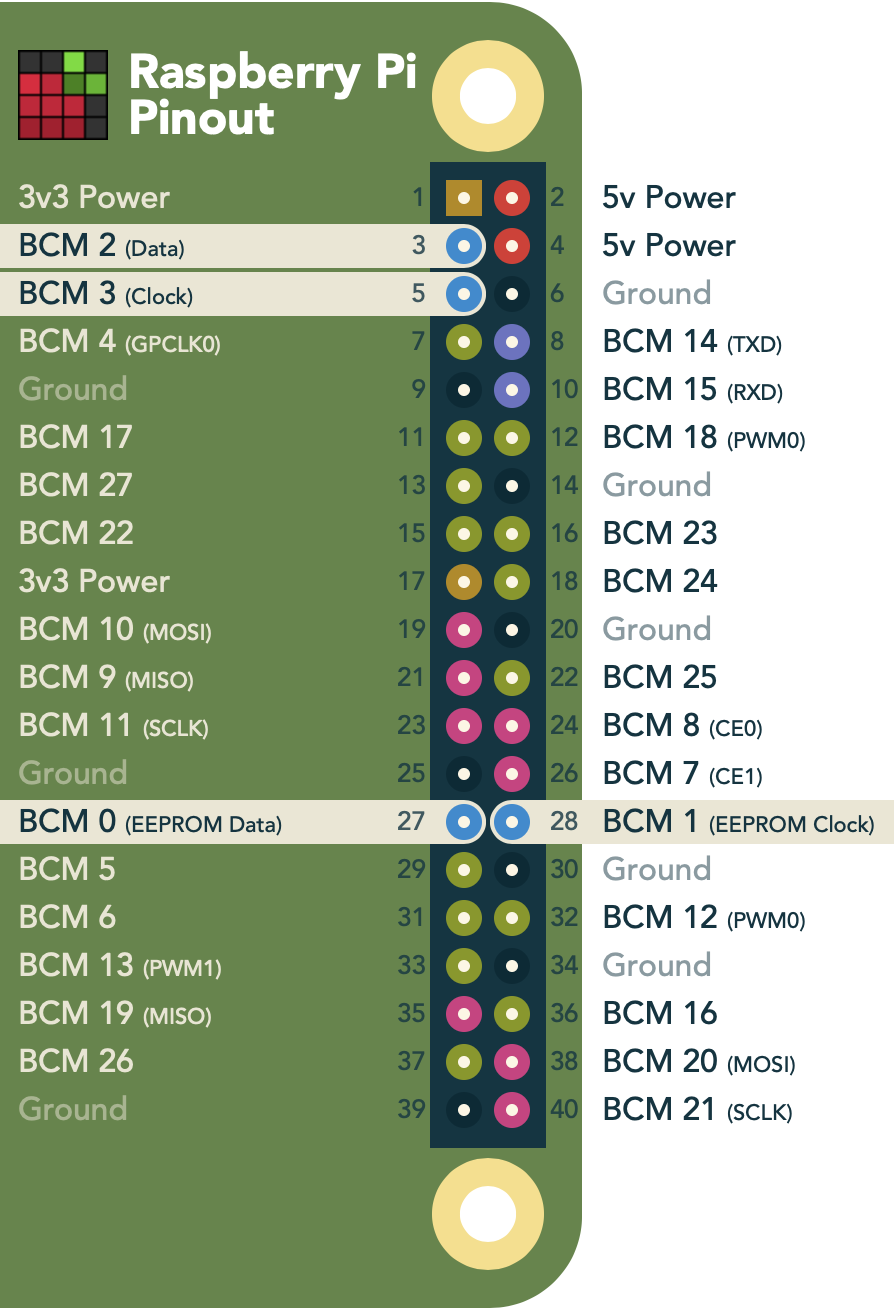
\includegraphics[height=2in]{IMAGES/rpi-pins-i2c}
      \end{subfigure}
      \begin{subfigure}{0.3\textwidth}
         \centering
         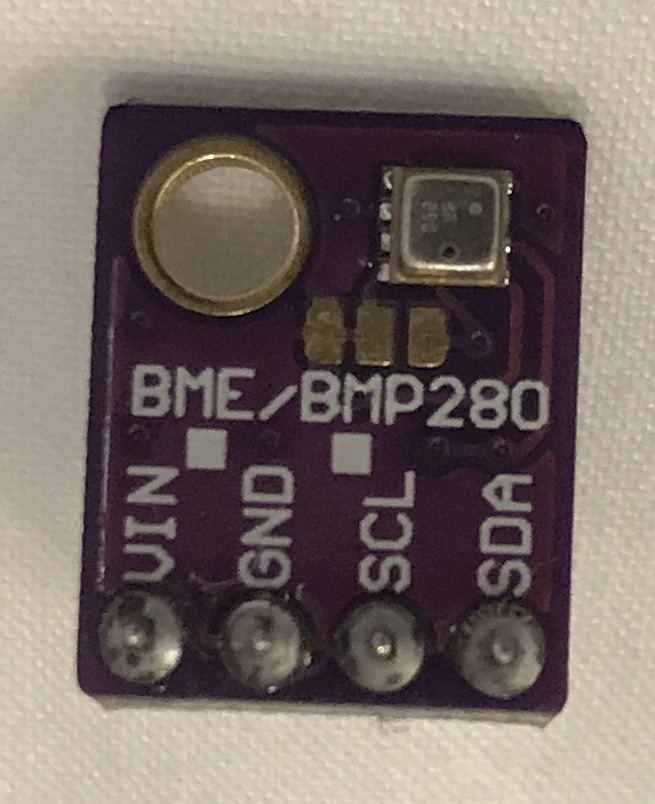
\includegraphics[height=2in]{IMAGES/BME280}
      \end{subfigure}
      \begin{subfigure}{0.3\textwidth}
         \centering
         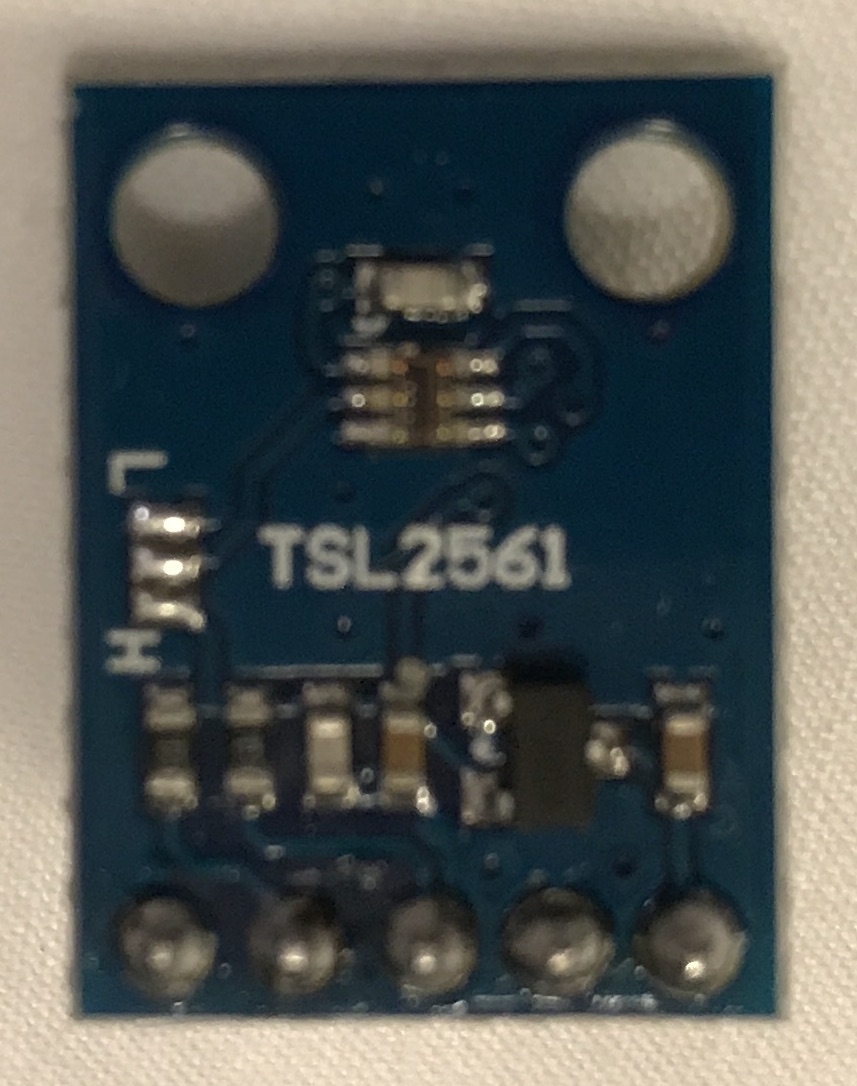
\includegraphics[height=2in]{IMAGES/TSL2561}
      \end{subfigure}
   \end{figure}
   \begin{itemize}
      \item We can access I2C devices via the I2C pins
      \item We will use the I2C bus to talk to the
	      \textbf{BME280 Environmental sensor}
	      and the \textbf{TSL2561 light sensor}
	      on the floral bonnet
   \end{itemize}
\end{frame}

\cprotect\note{

   You can learn more about the \textbf{raspberry-pi i2c pins} at pinout.xyz.

   \url{https://pinout.xyz/pinout/i2c}
}

